\section{Введение}
\subsection{Актуальность работы}

Кровь -- соединительная ткань внутри организма, она состоит из форменных клеток (эритроцитов, лейкоцитов, тромбоцитов), а так же из
водного раствора белков и свёртывающих веществ -- плазмы. Кровь под воздействием периодических сокращений сердечной мышцы 
движется по замкнутой системе сосудов, циркулируя от сердца и обратно. С точки зрения гидродинамики кровоток представляет 
из себя пульсирующее с низкой частотой течение мелкодисперсной суспензии в 
замкнутой системе каналов кругового сечения с эластичными стенками, осложнённое локальными эффектами ламинарно-турбулентного перехода.

Кровь, двигаясь по сосудам, испытывает сопротивление движению со стороны сосудов и из-за своей вязкости. Поэтому сердце вбрасывает 
кровь в сосуды под большим давлением. В аорте давление колеблется в диапазоне от 16~кПа при систоле до 10~кПа при диастоле. 
По мере движения крови давление в сосудистом русле падает. 
Скорость течения крови так же зависит от диаметра сосуда, удалённости сосуда от сердца, а также фазы сердечного цикла. 
Максимальных значений скорость достигает в аорте (до \texttilde$1$~м/с), а минимальных -- в капиллярах (около нуля).

Сложность разветвления кровеносных сосудов и вариации их размеров создают значительные трудности при решении задачи о течении крови. 
Математическое моделирование помогает  
пониманию сложностей кровотока. Эти модели позволяют описывать и строить физические процессы, происходящие 
в биологических системах. Это может быть полезно при выявлении, прогрессировании и лечении  различных сердечно-сосудистых заболеваний , 
а так же в проектировании и оптимизации медицинских устройств.

Кровь состоит из взвешенных в плазме 
(её рассматривают, как ньютоновскую жидкость) клеток крови, которые действуют друг на друга с некоторыми силами. 
Самые детальные методы моделирования заключаются в построении модели течения этих клеток как отдельных частиц в вязкой жидкости.
Описание такого типа методов можно подробнее изучить в ~\cite{Fedosov:2010,Fedosov:2008,Mehboudi:2001}. 
В некоторых моделях ~\cite{bessonov:2014,hosseini:2009} пренебрегают относительно мелкими и редкими -- тромбоцитами
(2--4~мкм в количестве 150--300 миллионов на 1~см$^3$) и лейкоцитами(4--20~мкм в количестве 4.5 -- 11 миллионов на 1~см$^3$), 
а моделируют лишь самые крупные из них -- эритроциты (7 -- 8~мкм в количестве 3.8 до 5.6 миллиардов клеток на 1~см$^3$).
Метод ресурсоёмкий, поэтому можно моделировать лишь небольшие участки кровотока (порядка 1~см и меньше) без ветвлений 
либо с одним - двумя ветвлениями.
Так же такая модель плохо реагирует на любые изменения в исходных данных, ведь свойства эритроцитов могут значительно изменяться, 
а модель строится под определённую их конфигурацию~\cite{Yamaguchi2010}. 
Соответсвенно, возникает необходимость прибегнуть к некоторым упрощениям постановки.

Можно не описывать индивидуальные частицы взвешенные в плазме, а обобщить их до вязкой неньютоновской жидкости с определёнными 
характеристиками, в которых отразить эффекты, связанные с наличием взвешенных в растворе частиц. Такой подход называют трехмерным моделированием.
Принципиальным моментом в формулировке такой постановки является выбор модели вязкости: например,
основанные на зависимости вязкости от гематокрита ~\cite{walburn:1976},
модель Максвелла \cite{thurston:1972},  модель Кассона ~\cite{moller:2006}.
Однако эти модели всё-таки требуют значительных вычислительных ресурсов, поэтому имеет смысл провести дальнейшее упрощение.

Наиболее простыми с точки зрения вычислительных ресурсов являются так называемые одномерные модели кровотока, в которых
пространственные характеристики осредняются по поперечному сечению, а трёхмерная дифференциальная
задача сводится к одномерной.

В некоторых случаях эти модели используют для постановки граничных условий в многомерных задачах. (ссыдки)
Но так же они могут и целиком моделировать кровеносную систему.(ссылки)

Такой подход к моделированию требует меньших вычислительных ресурсов, но при этом почти не уступает в 
точности другим моделям. О сравнении одномерных и многомерных моделей можно прочитать в ~\cite{FORMAGGIA:2001}.

{\bfВывод об актуальности}
Таким образом, несмотря на значительное увеличение доступных вычислительных мощностей и активное развитие детальных методов
численного моделирования гемодинамики, до сих пор полное описание системы кровообращения подробными моделями остаётся невозможным, 
а прямое или косвенное использование одномерных моделей для таких задач является безальтернативным выбором.
Поэтому развитие таких упрощённых моделей является актуальной задачей

\subsection{Обзор методов моделирования на основе одномерной постановки}

Принципиальным вопросом в построении одномерной модели кровотока является выбор зависимости давления в сосуде от площади его
поперечного сечения.

Можно использовать $N$ интегральных условий сохранения Бернулли выражающих непрерывность полного давления $P^l$:
\begin{equation}
    \label{eq:bernulli}
    \frac{\rho u^2_k}{2}+{p_k(A_k)}=P^l.
\end{equation}
Иногда для моделирования сопротивления потоку в местах стыка используют условия перепада давлений
с учётом сопротивления
\begin{equation}
    \label{eq:p-pressure}
    p_k\left(A_k\left(t,x_k\right)\right)-p^l(t)=\varepsilon_k R^l_k A_k(t,x_k)u_k(t,x_k),
\end{equation}
которое выражается через коэффициент $R^l_k$. Здесь $p^l$ -- давление в точке бифуркации \cite{bessonov:2014}.

Но общим способом замыкания системы является явное представление алгебраической зависимости
между давлением в сосуде и его площадью. Прямой подход к получению отношения $p(A)$ включает в себя точное одновременное измерение
давления и площади в разные моменты времени. Но такой метод не всегда удобен в реальности.
Качественный анализ физических экспериментов подтверждает, что функция $p(A)$ должна быть монотонной S-подобной кривой. 
Такая кривая удовлетворительно описывает состояния как круглого, так и эллиптического сечения. На рис.~\ref{ych} показана зависимость
зависимость давления в сосуде от его площади.


\begin{figure}[h]
    \centering
    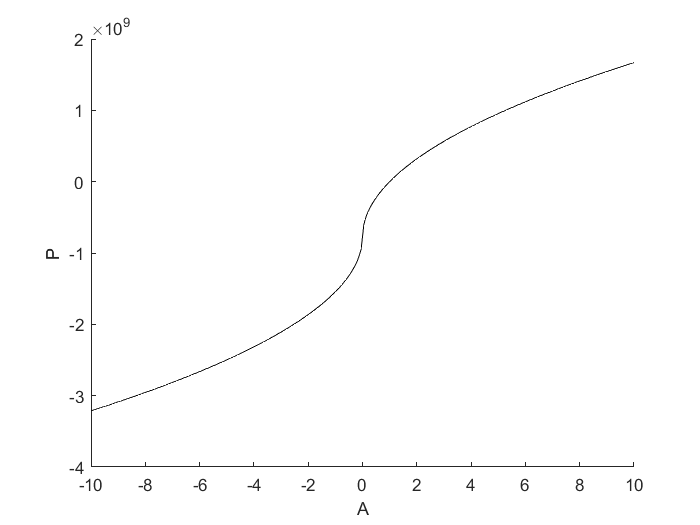
\includegraphics[width=0.5\linewidth]{PA.png}
    \caption{График зависимости давления от поперечного сечения внутри сосуда.}
    \label{ych}
\end{figure}

Для решения дифференциальных уравнений нужно выбрать подходящий метод пространственной аппроксимации области расчёта.

{\bf Метод конечных разностей} предполагает дискретизацию области на сетку точек и последующую аппроксимацию производных в управляющих
уравнениях с помощью конечных разностей. Этот метод часто используется в сочетании со схемой интегрирования по времени для решения 
полученной системы обыкновенных дифференциальных уравнений.

{\bf Метод конечных элементов}~\cite{TAYLOR1998} -- популярная численная схема. 
Он особенно хорошо подходит для моделирования сложных геометрий, таких как запутанная сеть артерий в человеческом теле. 
Однако он может быть вычислительно дорогим, особенно для больших и сильно разветвленных сетей. 

{\bf Метод быстрого преобразования Фурье}~\cite{Sazonov:2019} -- 
это подход, использующий быстрое преобразование Фурье для решения одномерных уравнений кровотока. 
Этот метод конкурирует с традиционными пространственно-временными численными схемами как по устойчивости, так и по скорости. 
Он может точно и эффективно обрабатывать сложные геометрические формы и высокоамплитудные волны. 
Однако он требует дальнейшего развития для учета вязкоупругих эффектов и потери массы крови из-за мелких ветвей. 

{\bf Метод разрывных конечных элементов Галеркина}~\cite{yao:2017} -- это еще одна численная схема, она сочетает в себе преимущества методов конечной разности и конечных элементов, 
обеспечивая баланс между точностью и вычислительными затратами. Однако он может быть более сложным в реализации и может
потребовать дополнительных вычислительных ресурсов для сопоставления расчетной и физической областей.

{\bf Метод конечных объемов с локальным временным шагом высокого порядка}~\cite{mueller:2015} предполагает решение управляющих уравнений 
с помощью метода конечных объемов высокого порядка и схемы локального шага по времени. 
Этот метод может быть особенно полезен для моделирования течения в сложных геометрических системах.

\subsection{Цель работы}
Целью настоящей работы является:
\begin{itemize}
\item разработка методики расчёта течения крови в одномерном приближении,
\item написание компьютерной программы для расчёта произвольной сети сосудов,
\item подбор оптимальных расчётных параметров: шагов по времени, пространству, количеству внутренних итераций,
\item верификация расчётной программы путём сравнения с численными и аналитическими результатами расчётов задачи в характерных модельных постановках от других авторов,
\item иллюстрация работы программы на примере сложной сети сосудов. Влияние изменения эластичных свойств одного из сосудов на интегральные характеристики течения 
      во всей системе.
\end{itemize}
